\documentclass[10pt, a4paper]{article}
\usepackage[a4paper, left=16mm, right=16mm, bottom=22mm, top=10mm]{geometry}
\usepackage{mathtools}
\usepackage{hyperref}
\usepackage{pgfplots}
\usepackage{graphicx}
\usepackage{multicol}

\hypersetup{
    colorlinks=true,
    linkcolor=blue,
    filecolor=magenta,      
    urlcolor=cyan,
}
\setlength{\columnsep}{6mm}

\title{DASH Policy Algorithm}
\author{Luca Crema}
\date{12/06/2020}

\begin{document}
    \maketitle
    \begin{multicols}{2}

    \section{Introduction}
    The following report will explore a custom policy
    for the \textbf{Dynamic adaptive streaming over HTTP}
    or \textbf{DASH}--like client protocol to reproduce a video
    to maximize the overall perceived video quality.

    \section{Environment simulation}
    To work on the client policy it has been set-up
    an environment that could simulate the communication 
    delays, the consumption of the downloaded video segments, and
    the eventual freezes.
    The simulation has been realized using \texttt{C++14} because
    it's a convenient object-oriented language and the one I know the
    most among the given options.

        \subsection{Segments}
        As defined in the DASH protocol the video is split into segments:
        for this simulation all of the segments have the same length,
        and each one has five levels of encoding available that differ
        in \textbf{bit size and quality}.

        \subsection{Client-Server}
        The client sequentially asks the policy for two things: the index of a
        segment and the encoding level to build a request to the server.
        The server will receive the request from the client and a bitrate value from
        a list then returns a response containing the time taken to transfer the
        chosen segment.
        \linebreak
        The client proceeds to store the downloaded segment in its buffer and
        updates the media playtime accordingly to how much time passed to get
        the response and how much buffered time it has, then it starts over.
        \linebreak
        To avoid the overwriting of already--played segments, the client has
        implemented protection that discards the downloaded segment if the current
        one in the buffer has already been played.

    \section{Quality metrics observations}
    We can notice that the penalty that weights the most in quality is long delays,
    this means that having long waiting times before the playout of the first segment
    is not profitable in the short term and shorter delays are preferable
    ($\exp(A+B+C) \gg \exp(A) + \exp(B) + \exp(C)$ for A,B,C big enough).

    \section{Custom policy}
    The policy starts by downloading the first segment at the highest possible encoding level
    to minimize initial waiting time.
    In every other case, it calculates the average bitrate of the
    previous $min(N_{avg}, L)$ elements (where $L$ is the number of segments in the buffer and
    $N_{avg}$ is a policy constant for the number of elements to calculate the average of)
    and underestimates it by multiplying it by $^2/_3$.
    \[R^{*}_{k} = \frac{2}{3} \times \frac{1}{N_{avg}}\displaystyle\sum_{i=L-N_{avg}+1}^{L}R_i\]
    There are now two possibilities:
    \begin{enumerate}
        \item There are still segments to download ($L < N_{tot}$).
        \item The buffer is full and we can improve the segments already in the buffer.
    \end{enumerate}

        \subsection{First case - buffer not full}
        The algorithm chooses to request the segment following the
        last one ($k = L+1$) in the buffer and calculates the encoding $c_k$ that gives the maximum
        $U_k$.
        If $B(t_{k-1}) - t^{'}_k = 0$, where $t^{'}_k$ is the amount of playout time consumed when
        downloading the k's element, it means that the video has frozen so
        the policy chooses the highest encoding level right away.
        \linebreak
        For this simulation the minimum encoding has been capped to 2 as it's been experimentally
        proven to be more efficient; I couldn't come up with a certain explanation but I
        suppose it's because lower encoding's bit sizes increase the probability for long
        waiting times when low--bitrate spikes occur.
        \linebreak
        The estimated delay time $\varphi^{*}_k$ is given by
        \[\varphi^{*}_k = \frac{M_k(c)}{R^{*}_{k}} - \frac{B(t_{k-1}) - t^{'}_k}{\lambda}\]
        where $\lambda$ is a policy constant that defines how many segments should be ready
        in the buffer at any given time.
        \linebreak
        The quality is then calculated using the given quality function:
        \[U_k = q_k(c_k) - \beta|q_{k-1}(c_{k-1}) - q_k(c_k)| - \exp(\gamma \varphi^{*}_k/T_s)\]

        \subsection{Second case - buffer full}
        The algorithm looks for a segment to improve starting from the
        one after what's currently playing, for each encoding available it calculates whether there's
        a valuable improvement and if it can be downloaded in time before that very segment
        has to be played, when it finds that segment with such encoding it chooses it to be 
        downloaded and overwritten.
    \end{multicols}

    \begin{figure}[h]
        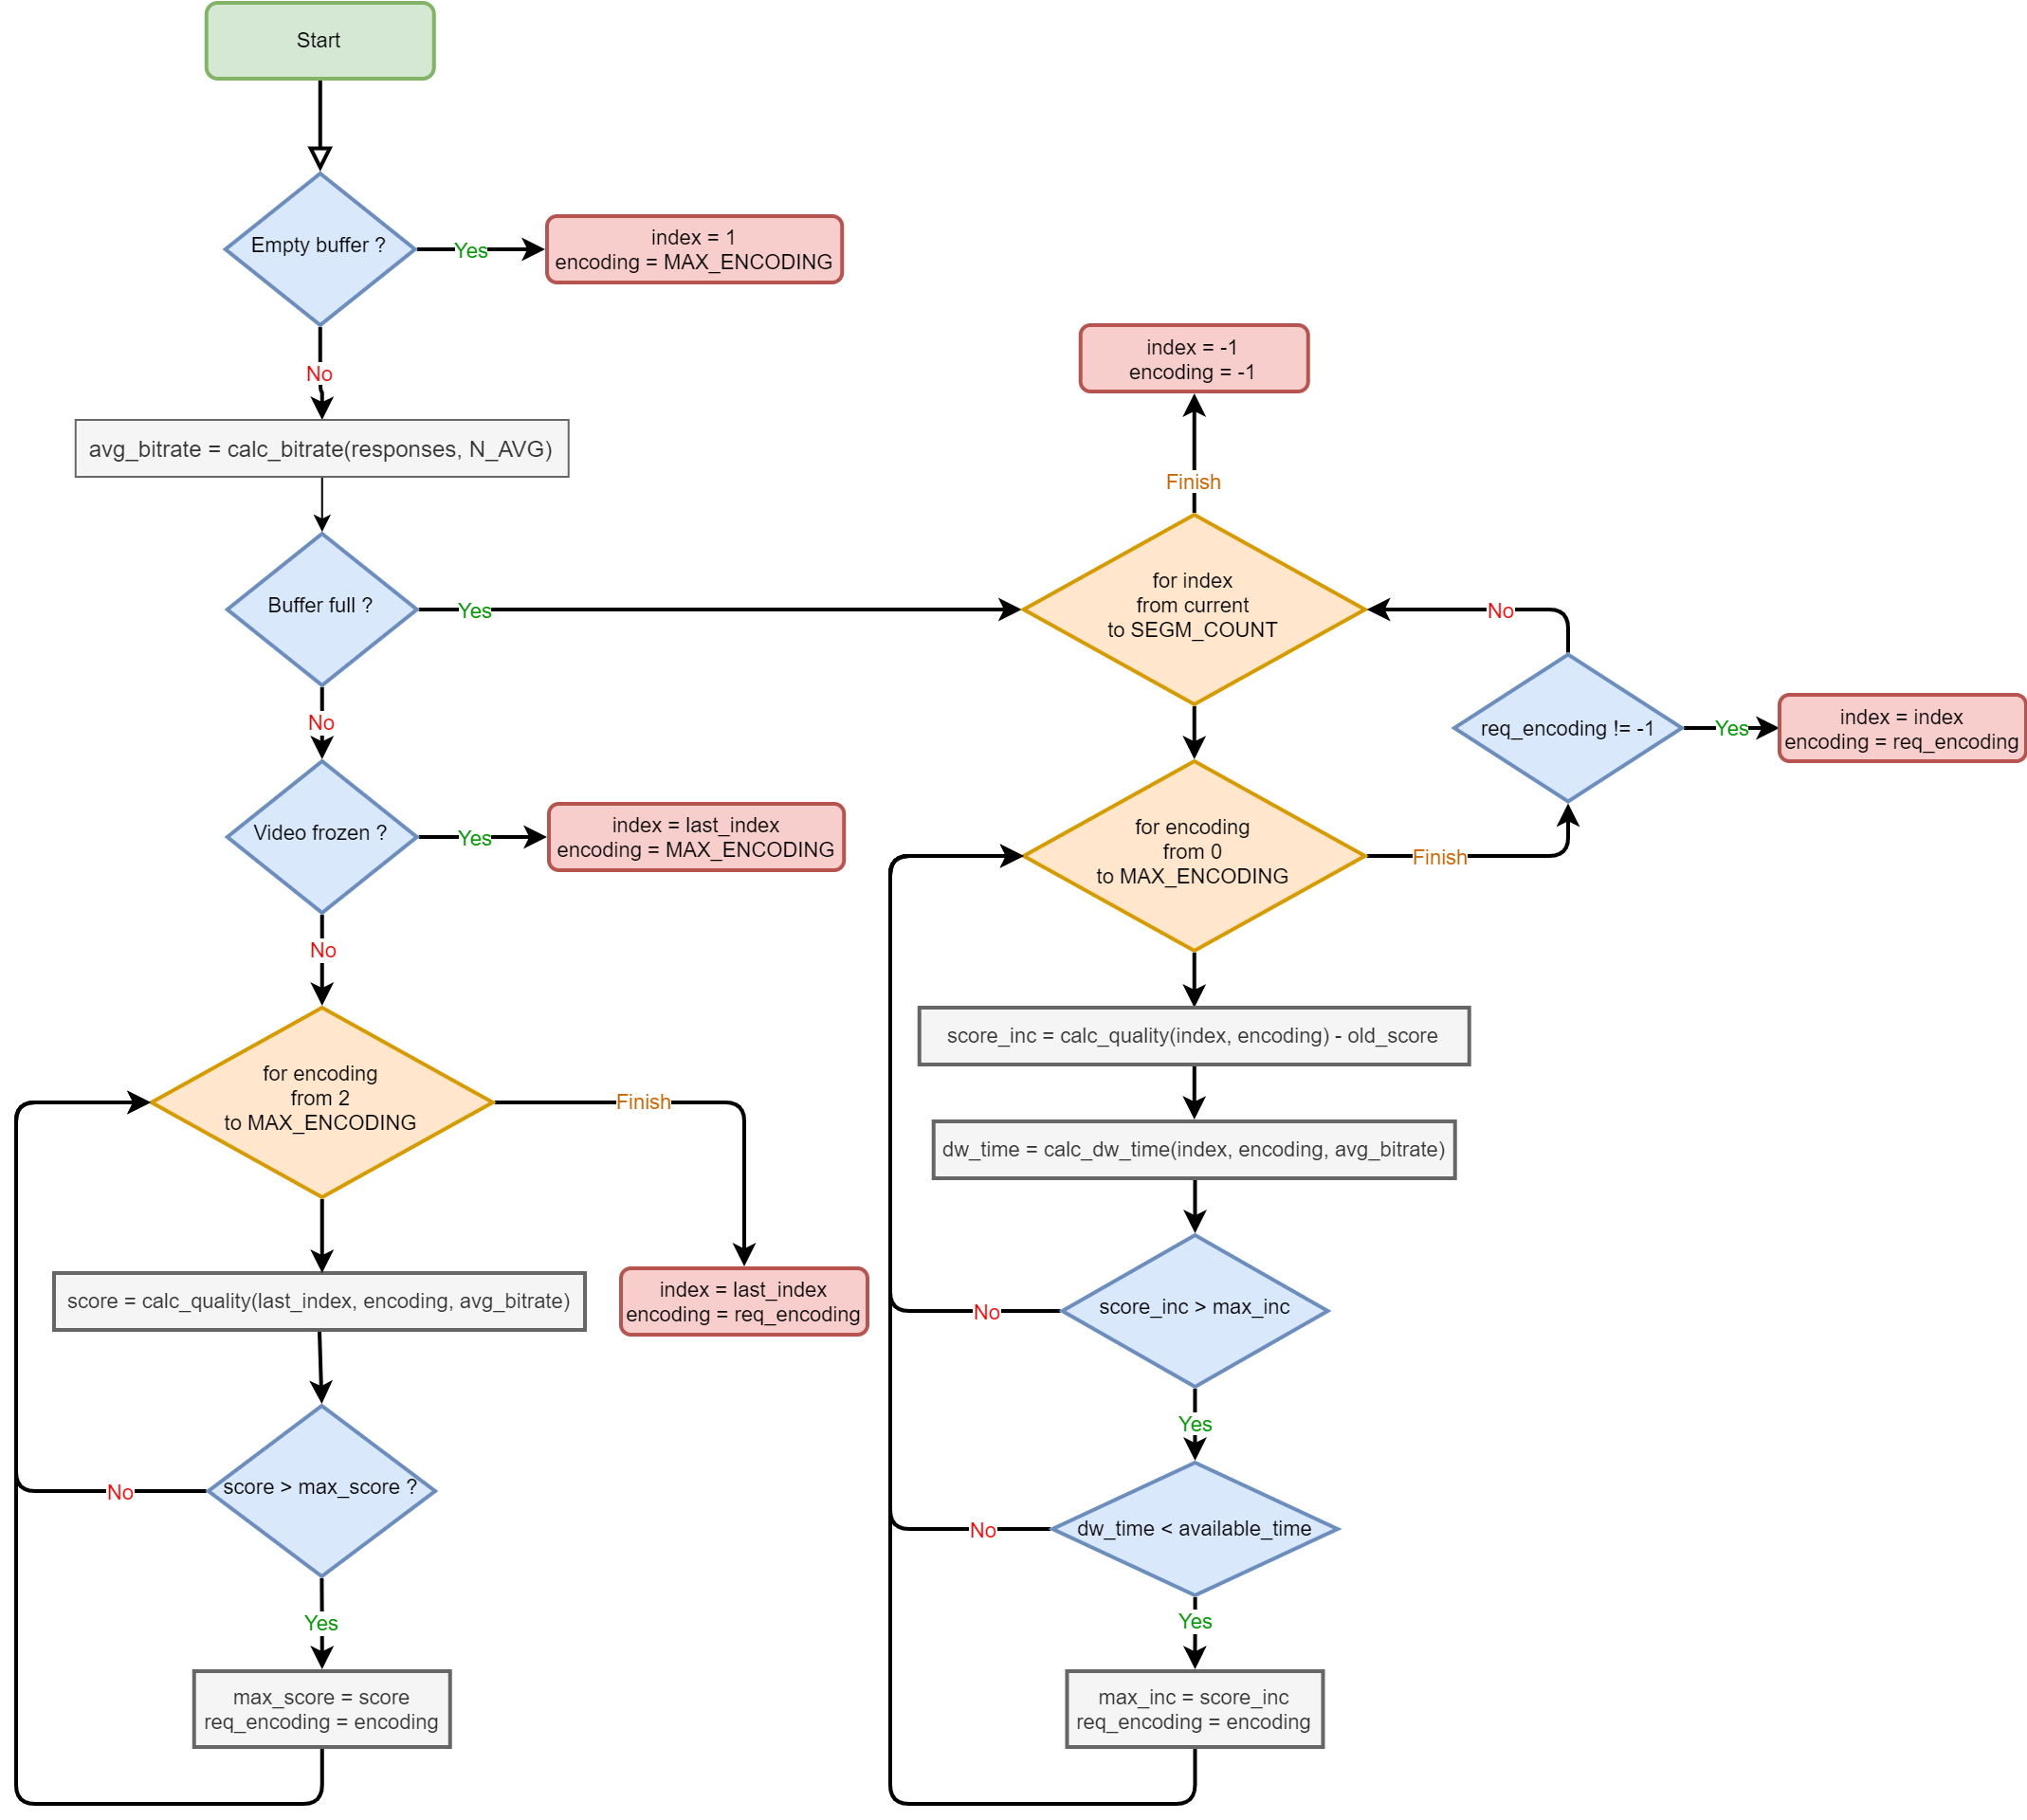
\includegraphics[width=\textwidth, height=17.5cm]{Policy_flowchart_2}
        \caption{Flow chart describing the algorithm.}
    \end{figure}

    \section{Performance}
    By testing with the given \texttt{MPD.txt} containing a
    Media Presentation Descriptor--like structure and 
    \texttt{channel.txt} containing a list of bitrates the
    final perceived quality of the user has been somewhere around
    the values of \textbf{34200} and \textbf{34500} (depending on some
    variables such as $N_{avg}$ and $\lambda$) which,
    by checking with other colleagues, is the best performance
    any of us managed to reach.
    To put it in perspective here are some other policy's performances:
    \begin{center}
        \begin{tabular}{ |c|c| } 
            \hline
            All encoding level 4 & 29000 \\ 
            All encoding level 3 & 33000 \\ 
            Professor's suggested policy & 30000 \\ 
            \hline
        \end{tabular}
    \end{center}
    Although it seems that the performance is similar to the trivial
    policies, it's exponentially harder to improve the algorithm and 
    gain quality after a certain value around 33500.
\end{document}